\subsection*{Updated Data Flow Diagrams}

\subsubsection*{Level 0 DFD}

Here is our updated top level DFD:

\begin{center}
  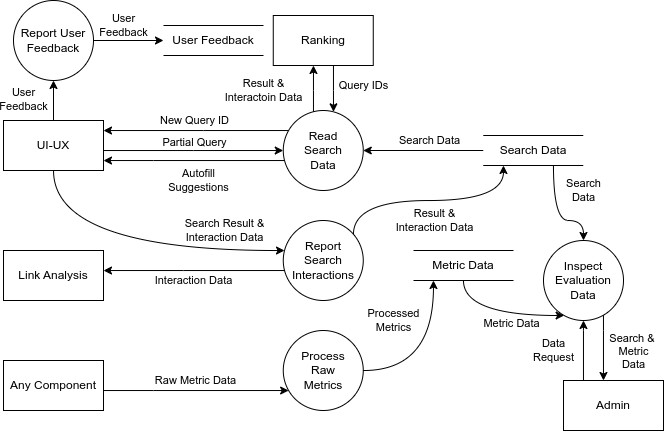
\includegraphics[scale=0.5]{DFDs/HighLevelDFD.drawio (1).png}
\end{center}
High Level Changes:
\begin{itemize}
  \item Ranking now asks for interaction data instead of us sending it to them on each query
  \item Added the Report User Feedback process for UI/UX
  \item Condensed read operations into one high level process
\end{itemize}

Report User Feedback is a simple operation, so no lower level DFDs are needed. The exact data received form UI/UX will be dumped to text files.

\subsubsection*{Level 1 DFDs}

\textbf{Read Search Data}

\medskip

Both the Ranking and UI/UX components will need to read data from our database in one way or another. UI/UX will need autofill suggestions and unique query IDs. Neither of these are directly stored, the way the interaction data that Ranking needs is, but they will still rely on the database contents to do this.

\begin{center}
  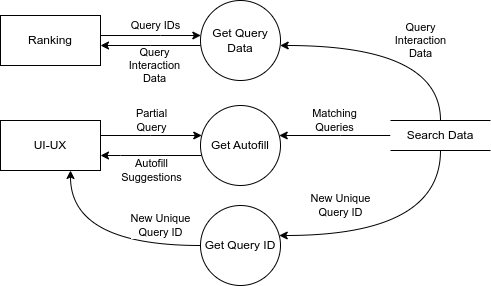
\includegraphics[scale=0.5]{DFDs/LowLevelDFDs-ReadSearchData.drawio.png}
\end{center}

\textbf{Report Search Interactions}

\medskip

After each query, the UI/UX team will send the user interaction data to us to be stored. Certain data will also be forwarded to Link Analysis for updating of the web-graph.

\begin{center}
  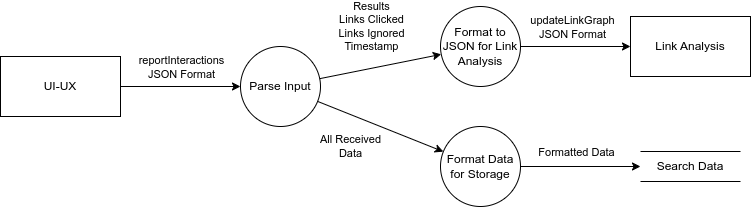
\includegraphics[scale=0.5]{DFDs/LowLevelDFDs-ReportSearchResults.drawio (2).png}
\end{center}
\subsection*{Functional Decomposition Diagrams}

\textbf{Process Raw Metrics}

\medskip

All components will be sending metrics data periodically. This will be in a variety of formats, but will be aggregated together for storage in the Metric Data Database.

\begin{center}
  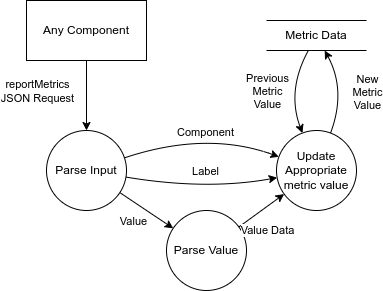
\includegraphics[scale=0.5]{DFDs/LowLevelDFDs-ReportMetric.drawio (1).png}
\end{center}

\textbf{Inspect Evaluation Data}

\medskip

The system administrator will have the opportunity to interact with our component through a command line interface to inspect the logged search history as well as the performance metrics. 

\begin{center}
  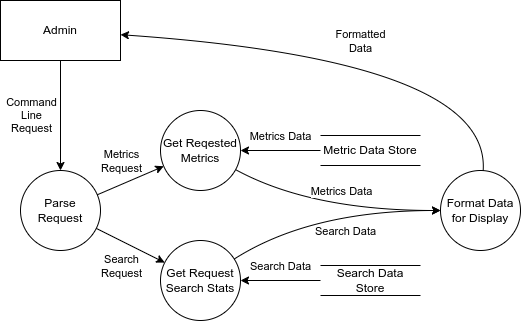
\includegraphics[scale=0.5]{DFDs/LowLevelDFDs-AdminView.drawio (1).png}
\end{center}

\subsubsection*{Level 2 DFD}

\textbf{Get Autofill}

\medskip

The other level 1 processes are relatively trivial, however autofill deserves a further expansion. We will attempt to correct typos, and search for similar queries (with and without typos). They will then be ranked and sent back to UI/UX.

\begin{center}
  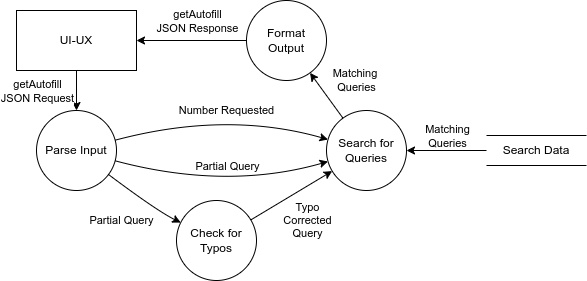
\includegraphics[scale=0.5]{DFDs/LowLevelDFDs-GetAutofill.drawio (2).png}
\end{center}

\subsection*{Architectural Divisions}

\subsubsection*{Outgoing Calls}

These are functions which we will call for other components to take action on.

\medskip

\textbf{Function:} \verb|updateLinkGraph():|

\smallskip

\textbf{Destination Component:} Link Analysis

\smallskip

\textbf{Data Format:} \begin{verbatim}
  {
    "updates": [
      {
        "results": [ <List of links shown to the user> ],
        "clicked": <index in the above list of the result the user clicked>
      },
      <More JSON objects with the above format>
    ]
  }
\end{verbatim}

\smallskip

\textbf{Side Effects:} The stored web-graph will be updated with this information. This is the responsibility of the Link Analysis team.

\subsubsection*{Incoming Calls}
These are the functions which other components will call for us to take action on.

\medskip

\textbf{Function:} \verb|reportMetrics():|

\smallskip

\textbf{Origin Component:} Any Component (All components will be calling this)

\smallskip

\textbf{Data Format:} \begin{verbatim}
  {
    "metrics": [
      {
        "label": <Label for the metric>
        "value": <Value for the metric>
      },
      <More metrics in the above format>
    ]
  }
\end{verbatim}

\smallskip

\textbf{Side Effects:} The metrics data that is sent will be stored for later use / display by a system Administrator.

\bigskip

\textbf{Function:} \verb|getAutofill():|

\smallskip

\textbf{Origin Component:} UI/UX

\smallskip

\textbf{Receive Data Format:} \begin{verbatim}
  {
    "num_suggestions": <Number of suggestions requested>,
    "partial_query": <The query which will be autofilled>
  }
\end{verbatim}

\textbf{Response Data Format:} \begin{verbatim}
  {
    "suggestions": [ <A list of suggestions for the complete query> ]
  }
\end{verbatim}

\smallskip

\textbf{Side Effects:} The above response will be sent to the UI/UX teams. They are responsible for showing these suggestions to the user.

\bigskip

\textbf{Function:} \verb|reportSearchResults():|

\smallskip

\textbf{Origin Component:} UI/UX

\smallskip

\textbf{Receive Data Format:} \begin{verbatim}
  {
    "query_ID": <Unique identifier of the query>
    "raw_query": <The exact query the user entered>,
    "results": [ <A list of results shown to the user> ],
    "clicked": <Index of the result the user chose in the above list>,
    "query_timestamp": <A timestamp for the query>
  }
\end{verbatim}

\smallskip

\textbf{Side Effects:} Our component will store all of this data, and call \verb|updateLinkGraph()|to propagate this information to the the web-graph.

\bigskip

\textbf{Function:} \verb|getQueryID():|

\smallskip

\textbf{Origin Component:} UI/UX

\smallskip

\textbf{Receive Data Format:} \begin{verbatim}
  {}
\end{verbatim}

\textbf{Response Data Format:} \begin{verbatim}
  {
    "query_ID": <Unique identifier of the query>
  }
\end{verbatim}

\smallskip

\textbf{Side Effects:} This query ID will never again be returned by \verb|getQueryID|

\bigskip

\textbf{Function:} \verb|getQueryData():|

\smallskip

\textbf{Origin Component:} Ranking

\smallskip

\textbf{Receive Data Format:} \begin{verbatim}
  {
    "query_IDs": [ <List of unique identifiers of queries> ]
  }
\end{verbatim}

\textbf{Response Data Format:} \begin{verbatim}
  {
    "queries": [
      {
        "query_ID": <Unique identifier of the query>,
        "results": [ <A list of results shown to the user> ],
        "clicked": <Index of the result the user chose in the above list>
      }, 
      <More queries in the above format>
    ]
  }
\end{verbatim}

\smallskip

\textbf{Side Effects:} None

\bigskip

\textbf{Function:} \verb|submitFeedback():|

\smallskip

\textbf{Origin Component:} Ranking

\smallskip

\textbf{Receive Data Format:} \begin{verbatim}
  {
    "label": <Some Label for the feedback>,
    "title": <Some title for the feedback>,
    "text": <Some text for the feedback>
  }
\end{verbatim}

\smallskip

\textbf{Side Effects:} The feedback is stored for admin viewing.

